%!TEX root = ../thesis.tex
%%--------------------------------------------------------------------------
%% STATE OF THE ARTS
%%--------------------------------------------------------------------------



% --------------------------------------------------------------------------- %
% ---------------------------------- INTRO ---------------------------------- %
% --------------------------------------------------------------------------- %


\section{Introduction}
\label{sec:sota_intro}
At the beginning of the development of the thesis we were mainly focused on the implementation of a module for OpenStack that would allow to implement different consolidation algorithms and test them to see their real impact on a cloud system in terms of resource allocation. During the first phases we faced with the problem of running, testing and benchmarking our code in an OpenStack environment: to deal with aspects like scheduling, VM placement, and consolidation we needed an highly configurable system that would allow us to run simulations and benchmark to evaluate the goodness of our solution. 
A common barrier to experimenting with cloud infrastructure is in fact the lack of access to a fully functional cloud installation. Although OpenStack can be used to create testbeds, it is not uncommon in literature to find works that are plagued by unrealistic setups that use only a handful of servers. Moreover, setting up a testbed is necessary but not sufficient. One must also be able to create repeatable experiments that can be used to compare one’s results to baseline or related approaches from the state of the art.
So we designed and develop a system to address this problem: we wanted it to be fully customizable to match different requirements and let the user customize a lot of aspect such as the structure of the environments, the number of compute nodes (the nodes that host the Virtual Machines), their fake characteristics or the OpenStack services to run. Secondly we needed a way to automatically simulate, in a repeatable way, the workload generated from user applications that normally run on an OpenStack installation. At last we realized that it would be very useful to show the real time data of the simulations to analyze the behavior of the system in different configurations.
Therefore we decided to develop aDock®, a suite of tools for creating performance, sandboxed, and configurable cloud infrastructure experimentation environments that developer, sysadmins and researchers can exploit to access a fully functional cloud installation of OpenStack.
For that reason this chapter is divided into two sections that describe the state of the arts of Virtual Machine consolidation and of Cloud test environments.


% ------------------------------------------------------------------------- %
% --------------------------- VMs consolidation --------------------------- %
% ------------------------------------------------------------------------- %

\section{Virtual Machine consolidation}
\label{sec:sota_vm_cons}

At its most basic essence, cloud computing can be seen as a means to provide developers with computation, storage, and networking resources on-demand, using virtualization techniques and the service abstraction \cite{Armbrust:2010ee}. The service abstraction makes the cloud suitable for use in a wide variety of scenarios, allowing software developers to create unique applications with very small upfront investments, both in terms of capital outlays and in terms of required technical expertise. Thanks to Cloud Computing, Internet software services have rightfully taken their place as important enablers in areas of great social importance, such as ambient assisted living \cite{Zhang:2011dq}, education \cite{Sultan:2010fd}, social networking \cite{Chard:2010eh}, and mobile applications \cite{Fernando:2013ip}.\\
Managing a Cloud Infrastructure, however, presents many unique challenges. For example, there has been a lot of focus in the last few years on Virtual Machine Placement and Server Consolidation, given the role they play in optimizing resource utilization and energy consumption \cite{Feller:2012kf}, \cite{Goudarzi:2012gw}. Virtual Machine (VM) Placement \cite{Meng:2010im}, \cite{Xu:2010df} defines how a cloud installation decides on which physical server to create a new virtual machine, when one is requested. Server Consolidation techniques \cite{Wuhib:2012vq}, \cite{Corradi:2014fe}, on the other hand, allow a cloud provider to perform periodical run-time optimizations, for example through the live migration of VMs. The goal is always to desist from having too many under-utilized hardware resources given a specific workload, and to achieve this without compromising the quality of service that is offered to the cloud’s customers.\\
Dynamic consolidation of Virtual machines is enabled by \textit{live migration}that is the capability of moving a running Virtual Machine between two physical hosts with no downtime and no disruptions for the user. Thanks to dynamic Virtual Machines consolidation is therefore possible to live migrate Virtual Machines from underutilized hosts to minimize the number of active hosts and remove Virtual Machines from hosts when those become overloaded to avoid performance degradation.

With regard to Virtual Machine Consolidation a lot of solutions, algorithms and techniques were proposed in literature \cite{He:2012jr}, \cite{Wuhib:2012vq}, \cite{Corradi:2014fe}, all with different approaches to the problem; we decided to focus on four interesting papers described in sections \ref{sec:sota_ga}, \ref{sec:sota_holistic}, \ref{sec:sota_game_theroy} and \ref{sec:sota_mutli_agent}. The section \ref{sec:sota_neat} is dedicated to the only attempted at the state of the art to apply Virtual Machine consolidation in the OpenStack world.

\subsection{Genetic Algorithm}
\label{sec:sota_ga}
In the paper \textit{Toward Virtual Machine Packing Optimization Based on Genetic Algorithm} \cite{Nakada:2009in} the authors explain how they modeled the problem of Virtual Machines consolidation as a bin packing problem and how they structured a Genetic Algorithm to deal with it. A Genetic Algorithm is an heuristic algorithm a type of techniques that are often used to address NP-hard problems as the bin packing problem. A GA is a model of machine learning that takes inspiration from the concept of evolution observed in biological environment from which it borrows a lot of terms such as Chromosome, Mutation or Population.\\
The paper in question defines the concepts of a Genetic Algorithm for the Virtual Machine packing problem as follows:
\begin{description}
  \item[Chromosome] It represents a physical node, and in particular the list of hosted virtual machines.
  \item[Crossover] They used a One-Point Crossover that randomly cut two chromosomes and mix them. They implemented a repair function to fix the inconsistent children thus obtained.
  \item[Mutation] They randomly exchange two position between them.
  \item[Initial Population Generation] They generate the initial population using a Minimal Generation Gap method.
  \item[Objecive Function] The unspecified objective function is said to be designed with some parameters and weights in mind such as SLA (Service level agreement) violations, number of active nodes and number of migrations applied.
\end{description}

The experimentation environment and the simulations tests are not described in a detailed way and there are no data results to prove the goodness of the approach. Still the idea of implementing a Genetic Algorithm to solve the consolidation problem is interesting and possibly very efficient and useful; for this reasons we decided to take inspiration from it and implement a Genetic Algorithm, to be applied in an OpenStack test environment deployed with aDock, as described in section \todo{aggiungere riferimento}.

\subsection{Holistic Approach}
\label{sec:sota_holistic}
\cite{Feller:2012kf}

\subsection{Game Theory Approach}
\label{sec:sota_game_theroy}
\cite{Xu:2014do}

\subsection{Multi-agent Virtual Machine Management}
\label{sec:sota_mutli_agent}
\cite{Anderson:2013bh}

\subsection{Neat}
\label{sec:sota_neat}
OpenStack, at the state of the art, provides a comprehensive and efficient Virtual Machines Placement system found, as described in chapter \ref{chap:openstack_devstack} \todo{inserire la sezione giusta}, in the \code{nova-scheduler} module; however, with regard to Virtual Machines Consolidation, OpenStack doesn't include any official solution or plans to include it.\\
The only project that tried to bring the Virtual Machine consolidation concepts to OpenStack is Neat\footnote{\url{github.com/beloglazov/openstack-neat}}, it is defined as a framework for dynamic and energy-efficient consolidation of virtual machines in OpenStack clouds \cite{beloglazov2014openstack}.\\
OpenStack Neat approaches the consolidation problem splitting it in four sub-problems~\cite[p.~3]{beloglazov2014openstack}:
\begin{itemize}
  \item  Deciding if a host is considered to be \textit{underloaded}, so that all Virtual Machines should be migrated from it, and the host should be switched to a low-power mode. 
  \item Deciding if a host is considered to be \textit{overloaded}, so that some Virtual Machines should be migrated from it to other active or reactivated hosts to avoid violating the QoS requirements.
  \item Selecting  Virtual Machines to migrate from an overloaded host.
  \item Placing  Virtual Machines selected for migration on other active or reactivated hosts.
\end{itemize}

\begin{figure}[!ht]
\centering{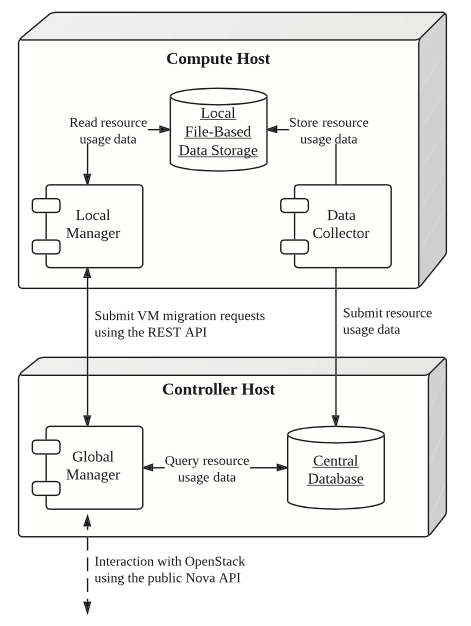
\includegraphics[width=\textwidth]{images/neat_arch.png}}
\label{fig:neat_arch}
\caption{The OpenStack Neat architecture \cite{beloglazov2014openstack}}
\end{figure}

In figure \ref{fig:neat_arch}~\cite[p.~7]{beloglazov2014openstack} it is represented the architecture of OpenStack Neat: it is mainly composed by a \textit{Global Manager} installed on the Controller node, a \textit{Local Manager}  and a \textit{Data Collector} both installed on every Compute node. The \textit{Global Manager} is responsible for making global management decisions such as mapping Virtual Machines instances to hosts, and initiating Virtual Machines live migrations; the \textit{Local Manager} makes instead local decisions such as deciding that the host is underloaded or overloaded and selecting Virtual Machines to migrate to other hosts; lastly the \textit{Data Collector}  is responsible for collecting data on the resource usage by Virtual Machines instances and hypervisors and then storing the data locally and submitting it to the central database, which can also be distributed.\\
One of the main characteristics of OpenStack Neat is that it is designed to be distributed and external to OpenStack, in fact it acts independently of the base OpenStack platform and applies Virtual Machines consolidation processes by invoking public APIs of OpenStack. For that reason it has to be installed separately from OpenStack, following the limited instructions present on the GitHub page of the project\footnote{\url{github.com/beloglazov/openstack-neat}} and can not take advantage of tools like DevStack (see \ref{chap:openstack_devstack} on page \pageref{chap:openstack_devstack}) that automates the deploy and configuration of an OpenStack installation. \\


% -------------------------------------------------------------------------- %
% ------------------------- CLOUD TEST ENVIRONMENT ------------------------- %
% -------------------------------------------------------------------------- %

\section{Cloud test environments}
\label{sec:sota_test_env}

In the cloud world is fundamental, as in any engineering field, to be able to test environment configurations and algorithms, both to analyze the behavior of tested code that integrates with a real environment and to benchmark and collect data for researches and experimentations. Unfortunately it can be expensive and complex to create and manage a cloud test environment in terms of time, resources and expertises, especially if the hardware resources like server machines or network infrastructures are limited. Fully understand and handle an OpenStack installation is not easy, especially for non sysadmins \todo{(Find a better way to say it)} like developers or researchers, it has indeed an high learning curve and often it is necessary a lot of time to achieve a good and desired result.
To reduce the impact of these complications are available some tools that make the process of setting up a cloud infrastructure experimentation environment more easy and manageable.
For these reasons and for the growing need of advanced system management configuration management tools, such as Chef and Puppet, have become increasingly mainstream. These tools provide domain-specific declarative languages for writing complex system configurations, allowing developers to specify concepts such as ``what software packages need to be installed'', ``what services should be running on each hardware node'', etc. More recently OpenStack has started collaborating both with Chef (see section \ref{sub:sota_chef}) and Puppet (see section \ref{sub:sota_puppet}) to create new means to configure and deploy fully-functional OpenStack environments on bare-metal hardware, as well as on Vagrant virtual machines. The combination of a system management tool, like Chef or Puppet, and Vagrant can be used to setup a virtualized experimentation environment. However, these are complex sysadmin tools that require strong technical skills.\\
Below we are presenting them highlighting their main features and their strengths and weaknesses with respect to our thesis topic.

\subsection{Vagrant}
\label{sub:sota_vagrant}
Vagrant\footnote{\url{www.vagrantup.com}} is a virtualization framework for creating, configuring and managing development environments, written in Ruby, that allows to  virtual development environments. It is a wrapper around virtualization software such as VirtualBox, KVM, VMware and could be used together with configuration management tools such as Chef and Puppet.
Thanks to an online repository \footnote{\url{www.vagrantcloud.com}} it is possible to automatically download a Vagrant Box and run it with a single command: \code{vagrant up vagrant-box-name}.
It is also possible to create and configure custom Vagrant Box by simply writing a Vagrantfile:
\begin{lstlisting}[language=Ruby]
box      = 'trusty64'
url      = 'http://files.vagrantup.com/precise32.box'
hostname = 'customtrustybox'
domain   = 'example.com'
ip       = '192.168.0.42'
ram      = '2048'

Vagrant::Config.run do |config|
  config.vm.box = box
  config.vm.box_url = url
  config.vm.host_name = hostname + '.' + domain
  config.vm.network :hostonly, ip

  config.vm.customize [
    'modifyvm', :id,
    '--name', hostname,
    '--memory', ram
  ]
end
\end{lstlisting}
Provisioners in Vagrant allows to automatically install and configure software in a Vagrant Box as part of the ``vagrant up'' process, therefore you can start with a base Vagrant Box, adapt it to your needs and eventually share it with other developers who can reproduce the same virtual development environment.
Vagrant in combination with configuration management software such as Chef and Puppet is used to create repeatable and easy to setup development and test environments that rely on Virtual Machines.


% ---------------------------------- CHEF ---------------------------------- %

\subsection{Chef}
\label{sub:sota_chef}

\subparagraph{Description}
\label{subp:sota_chef_desc}

Chef\footnote{\url{www.chef.io}} is a configuration management tool used to streamline the task of configuring and maintaining servers in a cloud environment and can be integrated with cloud-based platforms such as Rackspace, Amazon EC2, Google Cloud Platform, OpenStack and others. It is written in Ruby and Erlang and uses a domain-specific language (DSL)\footnote{A programming language specialized to a particular application domain.} for writing configuration files called ``recipes''. ``Recipes'' are used to define in a declarative way the state of certain resources and define everything that is required to configure different parts of the system: they can contain the definition of software that should be installed and all the required dependencies, services that should be running or files that should be written. Given a ``recipe'' Chef ensures that all the software is installed in the right order and that each resource state is reached, eventually correcting those resources in a undesired state; ``recipes'' can be collected into ``cookbooks'' to be more maintainable and powerful. In addition Chef offers a centralized hub, called Chef Supermarket\footnote{\url{supermarket.chef.io}}, that collects a large number of ``cookbooks'' from the community freely downloadable.\\
A base installation of Chef is composed by three main components, a \code{chef-server} that orchestrates all the Chef processes, multiple \code{chef-client} found on all the servers, and the user workstation that communicates with the Chef Server to launch commands.\\
To simplify the communication with the \code{chef-server} Chef provides a command-line tool called Knife that helps users to manage nodes, ``cookbook'' and ``recipes'', and the majority of possible operations.

\subparagraph{Chef and OpenStack}
\label{subp:sota_chef_openstack}

Chef and OpenStack can be combined and used together in different ways, many of which have a different goal compared to our thesis. Is it possible in fact to deploy and manage a production OpenStack installation running on multiple servers and supervised by a Chef Server using the subcommand \code{knife openstack} to control the OpenStack APIs through Chef and thus instantiate new physical servers with a chef-client installed or turn them off (\code{knife openstack server create / delete}).
In this situation you can achieve a ``1 + N'' configuration that is one OpenStack Controller and N OpenStack Nodes, and the OpenStack services are predefined and you cannot configure an ad hoc configuration.
Therefore an ``All-in-One Compute'' configuration can be chosen where all the OpenStack services are installed on a single node.\\
These configurations can be achieved with the help of Vagrant that will cover all the steps to install OpenStack on a virtual machine and configure all its services (excluded Block Storage, Object Storage, Metering, and Orchestration). Within the OpenStack chef-repo\footnote{\url{https://github.com/stackforge/openstack-chef-repo}} there is a Vagrantfile that configure a VirtualBox virtual machine that will host and All-in-One installation. Here is a part of it:

\begin{lstlisting}[language=Ruby]
machine 'controller' do
  add_machine_options vagrant_config: controller_config
  role 'allinone-compute'
  role 'os-image-upload'

  chef_environment 'vagrant-aio-nova'
  file('/etc/chef/openstack_data_bag_secret',
       "#{File.dirname(__FILE__)}/.chef/encrypted_data_bag_secret")
  converge true
\end{lstlisting}

Of course it is possible to setup a ``1 + N'' configuration using different Vagrantfile to create and configure one VM to host the Controller and N VMs to host the Compute nodes. However it is unlikely to succeed in running a lot of VMs on the same host especially if they will contain a fully functional OpenStack installation as a Virtual Machine typically require a significant amount of resources to operate.

\todo{\dots  Insert timing to install OpenStack with Chef\dots}

\subparagraph{Pro and Cons}
\label{subp:sota_chef_pro_cons}

Chef, as seen, is therefore a very powerful tool to create, manage and configure cloud environments and offers a lot of functionalities to structure the desired architecture. In combination with Vagrant is also useful to setup test environments for development or research purposes.\\
However, with regard to this last aspect, it has several limitations:
\begin{itemize}
\item \textit{Heaviness}: due the greed of resources of a Virtual Machine is very difficult to achieve a ``1 + N'' configuration for development or research purpose on a single machine. On the other hand the ``All-in-One Compute'' solution that allows a full OpenStack installation on a single Virtual Machine is very simplistic and doesn't represent a real environment setting as it runs all the OpenStack services on a single node.
\item \textit{Lack of customization}: at the state of the art all of the described solutions install both the Controller node and the Compute node with a predefined set of installed service (in particular are installed all the OpenStack service excluded Object Storage, Metering, and Orchestration) so it is not possible to setup the environment with more or less services or new ones (as in our case).
\item \todo{think others\dots}
\end{itemize}


% ---------------------------------- PUPPET ---------------------------------- %


\subsection{Puppet}
\label{sub:sota_puppet}

\subparagraph{Description}
\label{subp:sota_puppet_desc}

Similarly to Chef (described in section~\ref{sub:sota_chef}) Puppet\footnote{\url{www.puppetlabs.com}} is a configuration management system that allows you to define the state of a cloud infrastructure and then it automatically enforces the correct state.\\
Puppet uses a declarative model where are defined the resource states and (likewise Chef) it's manifest files are written in a Ruby-like DSL. In these manifest files are defined the configurations, the nodes and how the configurations apply to nodes. Again Puppet will take care of ensuring that the system reaches the expected state. All these files are enclosed in ``modules'', a self-contained bundles of code and data easy to share and reuse. There are a large amount of them on Puppet Forge\footnote{\url{forge.puppetlabs.com}} repository.\\
Puppet is structured in master-slave architecture: the master (that can be one or machines) serves the manifests and the files, and the clients polls the master at specific intervals of time to get their configurations so that the master never pushes nothing to them. This structure uses the ``Puppet master'' and ``Puppet agent'' applications.


\subparagraph{Puppet and OpenStack}
\label{subp:sota_puppet_openstack}

As seen for Chef, Puppet can be very useful when dealing with OpenStack installation and maintenance. To configure and deploy an OpenStack infrastructure with the help of Puppet exists a set of ``modules'' freely downloadable from Puppet Forge that simplifies most of the operations such as OpenStack instances provisioning, configuration management and others.
The module is \code{puppetlabs-openstack}\footnote{\url{github.com/puppetlabs/puppetlabs-openstack}} and allows to deploy both a multi-node and an all-in-one installation. Compared to Chef, with regard to OpenStack, Puppet is a bit more flexible because it allows you to control in more details the OpenStack services installed on every node; for example you can, combining the following instructions, in the Puppet's manifest file of a node different results can be achieved:

\textit{Controller node:}
\begin{lstlisting}[language=Ruby]
node 'control.localdomain' {
  include ::openstack::role::controller
}
\end{lstlisting}

\textit{Controller node:}
\begin{lstlisting}[language=Ruby]
node 'storage.localdomain' {
  include ::openstack::role::storage
}

node 'network.localdomain' {
  include ::openstack::role::network
}

node /compute[0-9]+.localdomain/ {
  include ::openstack::role::compute
}
\end{lstlisting}

Obviously, in the same way for Chef, it is possible to configure multiple nodes to run in multiple Virtual Machines configured and launched with Vagrant and deploy the various OpenStack components with \code{puppetlabs-openstack}. This solution, as said earlier, is difficult to achieve on a machine with a limited amount of resources, and also on more powerful server is however slightly extensible.

\subparagraph{Pro and Cons}
\label{subp:sota_puppet_pro_cons}
Puppet is an extremely powerful and mature tools for automated cloud infrastructure deploying: it streamlines the entire process automating every step of the software delivery process.\\
However from our point of view it is more relevant to how it behave when a single developer or a researcher needs to deploy a cloud infrastructure within a single machine with limited amount of resources (a development workstation for example) or he/she has a little sysadmin skills (\todo{find better way}) and want to run test for developing or researches purposes. With regard to this aspect Puppet used with Vagrant has some key limitations:

\begin{itemize}
\item \textit{Heaviness}: A single Virtual Machine need generally a remarkable amount of resource, especially to host an OpenStack installation; for this reason it is very unlikely to be able to run the number of Virtual Machines needed to deploy a realistic multi-node installation of OpenStack on a single machine without compromising its usage. The all-in-one instead is frequently not sufficiently realistic, especially when testing algorithms or portion of code that involves multiple nodes.
\item \todo{think others\dots}
\end{itemize}

% ---------------------------------- CHEF ---------------------------------- %

\subsection{Docker}
\label{sub:sota_docker}
Docker\footnote{\url{www.docker.com}} is an open platform for developers and sysadmins to build, ship, and run distributed applications. Its core is the Docker Engine: it exploits Linux containers to virtualize a guest Operating System on an host one avoiding the considerable amount of resources necessary to run Virtual Machines.\\
The main difference between the Docker solution and the Virtual Machine one lies in the way in which the hypervisor and the Docker Engine manage the guest Operating System. A Virtual Machine, as shown in figure ~\ref{fig:docker_vm} on page~\pageref{fig:docker_vm}, hosts a complete Operating System including application, dependency libraries, and, more important, the kernel; otherwise the Docker Engine runs as an isolated process in userspace on the host operating system and allows all the guest containers to share the kernel. Thus, it enjoys the resource isolation and allocation benefits of Virtual Machines but is much more portable and efficient; for our goals this aspect represents the possibility to run at the same time a larger number of containers compared to what we are able to achieve with Virtual Machines and also to ship pre-built images of our modules \todo{Better way...}.\\
To configure and then build a container image you have to write a Dockerfile that is a text document containing all the commands which you would have normally executed manually in order to take the container to the desired state and then call \code{\$ sudo docker build .} from the directory containing the file. The command \code{\$ sudo docker run} will finally launch the container that will be almost instantly running.\\
Moreover Docker offers an online platform called Docker Hub\footnote{\url{hub.docker.com}} where you can upload both Dockerfile and pre-built container images to streamline the sharing process.
    
\begin{figure}[!ht]
\centering{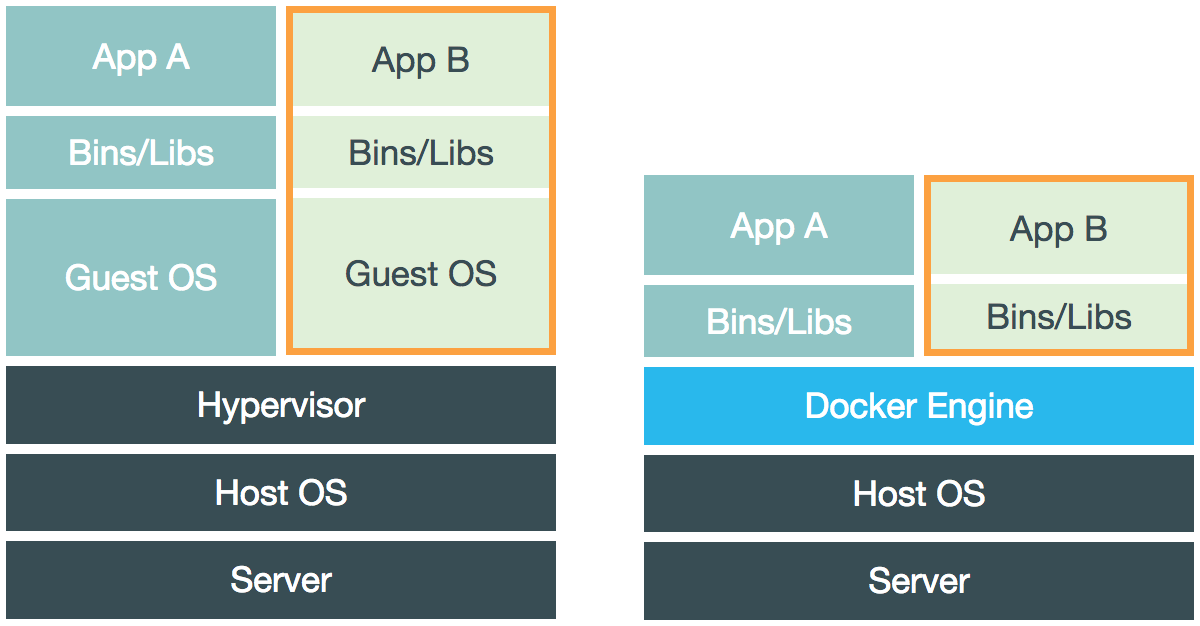
\includegraphics[width=\textwidth]{images/docker_vs_vm.png}}
\label{fig:docker_vm}
\caption{Hypervisor and Docker Engine}
\end{figure}

% ------------------------------- DOCKENSTACK ------------------------------- %

\subsection{Dockenstack}
\label{sub:sota_dockenstack}
One of the first an attempts to create a cloud test environments based on OpenStack and Docker is a Dockenstack\footnote{\url{github.com/ewindisch/dockenstack}}. It is an independent and not actively supported project, but is a good starting point to show the potential derived from using Docker.\\
The project is basically composed by a Dockerfile and a bunch of scripts that will setup and configure an OpenStack installation using DevStack (\todo{shall we talk about it in the intro?}) in a Docker container.\\
A pre-built image is available on Docker Hub, so with the command \code{docker run -privileged -t -i ewindisch/dockenstack} Docker will automatically download and run the container.\\
This made it a good solution for beginners wanting to learn OpenStack, but inadequate for advanced experiments, such as experiments regarding Virtual Machines placement and server consolidation algorithms.

